%%%%%%%%%%%%%%%%%%%%%%%%%%%%%%%%%%%%%%%%%
% Structured General Purpose Assignment
% LaTeX Template
%
% This template has been downloaded from:
% http://www.latextemplates.com
%
% Original author:
% Ted Pavlic (http://www.tedpavlic.com)
%
% Note:
% The \lipsum[#] commands throughout this template generate dummy text
% to fill the template out. These commands should all be removed when 
% writing assignment content.
%
%%%%%%%%%%%%%%%%%%%%%%%%%%%%%%%%%%%%%%%%%

%----------------------------------------------------------------------------------------
% PACKAGES AND OTHER DOCUMENT CONFIGURATIONS
%----------------------------------------------------------------------------------------

\documentclass[12pt]{article}

\usepackage{fancyhdr} % Required for custom headers
\usepackage{lastpage} % Required to determine the last page for the footer
\usepackage{extramarks} % Required for headers and footers
\usepackage{graphicx} % Required to insert images
\usepackage{lipsum} % Used for inserting dummy 'Lorem ipsum' text into the template
\usepackage{wrapfig}
\usepackage{enumitem}

\usepackage[explicit]{titlesec}

\usepackage[export]{adjustbox}

% Margins
\topmargin=0in
\evensidemargin=0in
\oddsidemargin=0in
\textwidth=6.5in
\textheight=9in
\headsep=0.5em 

\linespread{1} % Line spacing

% list spacing
\setlist{nosep}

% caption spacing
\setlength\belowcaptionskip{-5pt}

% \bibliographystyle{plain}

\titleformat{\section}
  {\bfseries}{\thesection}{0em}{#1}
\titlespacing*{\section}{0em}{0em}{0em}[0em]

% Set up the header and footer
\pagestyle{fancy}
\lhead{\AuthorName} % Top left header
\chead{\Title} % Top center header
\rhead{\Subject} % Top right header
\fancyfoot{}
% \lfoot{\lastxmark} % Bottom left footer
% \cfoot{} % Bottom center footer
% \rfoot{Page\ \thepage\ of\ \pageref{LastPage}} % Bottom right footer
\renewcommand\headrulewidth{0.4pt} % Size of the header rule
% \renewcommand\footrulewidth{0.4pt} % Size of the footer rule

\setlength{\parskip}{0.4em}
\setlength\parindent{0pt} % Removes all indentation from paragraphs


\newcommand{\Title}{Project Narrative} % Assignment title
\newcommand{\Subject}{NSTRF 2016}
\newcommand{\AuthorName}{Colin Rennie} % Your name

\begin{document}
\newpage

\begin{center}
{\bf Planning and Control for Tethered Cave Exploration }

\end{center}

%---------------- Introduction ------------------
%Tethered Robot Importance 
%Planetary exploration
%Situations needing tethers for science targets
%Communications


%---------------- Proposed Research ------------------

Inspired by the variety of science missions that would be achievable
using a tethered robot but not using a more traditional wheeled rover, 
scientific research in this area has produced substantial progress in 
recent past. This research has focused on several different designs of
tethered robots including notable examples of an eight-legged walking robot attached to a 
stationary base and two-wheeled differential drive pairs of tethered robots. Both designs
feature an actuated winch or spooled tether used for communication and/or 
stability while repelling uneven and difficult terrain.

%Dante II (& lemur II?)
The Dante II robot design consisted of eight legs for locomotion and an 
actuated winch for repelling down steep and difficult terrain. Both actuation 
mechanisms were attached to 
a base frame with a sensor arch protruding from the top of the structure. A variety of
sensing equipment, including a pan/tilt camera and a laser range finder,
 were attached to the arch in order to retrieve and transmit data from remote
 locations. In 1994 the system was deployed into Mount Spurr, an active volcano, 
 in order to record data for further scientific analysis. The robot's control 
 during this time was a combination of supervised autonomous motions and remote
 teleoperation. Aside from a failure where the robot incurred a lateral force at its contact
point with the tether, fell over and was not able to correct itself,
 the 5-day mission was regarded as a success in showing the capabilities of robotic
 systems to act as ``surrogate scientists'', exploring where humans would not otherwise
 be able. 

%Axel platform (+picture)
%Motion planning solution
%Problems
%   Quasi-static, no cable friction with ground assumed
%   solution is planar, over-simplifying the environment
%   assumes static anchor point (base unit)
More recently, NASA's Jet Propulsion Laboratory has been working on a two-wheeled
differential drive tethered robot, appropriately named ``Axel''. The Axel robot 
design features collapsible, paddled wheels, making the system more appropriate for longer 
and more remote missions as this design is more robust to issues such as high-centering and 
failures such as that encountered by Dante II. The tether mechanism is connected to the axel 
between the two wheels and is actively spooled as the wheels move relative to the body of the robot. 
Two variants of the system are presented: one in which Axel is attached to a stationary anchor point, 
and a second where two Axel robots are tethered together and deployed via a central support beam. 

The open question in either design variation is how to plan autonomous descent and corresponding 
ascent paths for the deploying tethered Axel robot in uneven, rocky, extra-planetary terrains. 
A solution framework is presented which projects this complex problem to a two-dimensional plane and, 
building on foundational work addressing the tether constraint problem from a computational geometry 
perspective, extends this work to produce ``stable'' paths by deriving equations of motion arising from 
the constraints of the Axel robot. The resulting algorithm first plans the more difficult ascent path and
uses this solution to limit its search for viable descent paths lying in the same homotopy class. 





%---------------- Proposed Research ------------------

{\bf Introduction \\}

\vspace{-0.15in}In this proposal, we consider as an example the case of an exploratory rover which has been deployed into a cave by a main robotic base unit. The tether we consider is a spooled, flexible tether which serves two primary purposes: (1) to deploy into and retrieve the exploratory rover from constrained environments with scientific value in terms of mission objectives and (2) for communication between the exploratory and base units. For the sake of this proposal, we imagine that both rover units at either end have a rotational joint in order to actuate the tether. We also imagine both units to be equipped with a means of sensing forces imparted upon the rovers by the tether (e.g., force/torque sensors). \\

{\bf Research Problem 1: Coordinated maneuvering of a soft tether \\}
\begin{wrapfigure}{r}{0.5\textwidth}
  \begin{center}
    \vspace{-0.5in}
    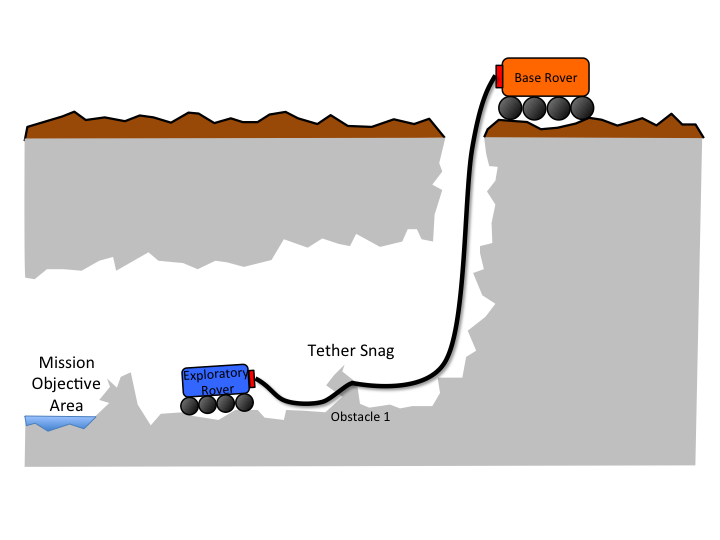
\includegraphics[width=0.48\textwidth, right]{cave_exploration}
  \end{center}
  \vspace{-0.5in}
  \label{fig:cave}
  \caption{A base rover (orange) has deployed an exploratory rover counterpart (blue) into a cave to achieve scientific mission objectives. Pictured, while in route to the mission objective region, the tethered communications cable becomes snagged on an unknown obstacle.}
\end{wrapfigure}
\vspace{-0.15in}

Exploring unknown and remote environments such as a cave on a remote planet or satellite involves a substantial amount of uncertainty in the topology of the terrain to be explored. When deploying an exploratory tethered rover into such an environment, the probability of unintentionally wrapping the tether around an obstacle increases substantially \ref{fig:cave}. This ``snag'' in the tether would then impair the robot by reducing its reachable workspace and may render scientific mission areas unreachable. 

Addressing this problem in our current example, our first task would be to build a sensing module capable of robustly identifying such situations by using the on-board force/torque sensors and using this information to identify the approximate position of the obstruction relative to the two rovers. In order to then untangle the tether, a promising strategy is to actuate the base rover's tether coupling, producing a traveling waveform through the body of the tether (capable of knocking the tether loose) while simultaneously communicating these controls to the exploratory rover. The challenge in this strategy however, is that once the cable is free it is likely to impart a substantial force on the exploratory robot, potentially resulting in dangerous jerking of the rover in a partially known environment. 

We would then propose to solve this problem by propagating in response a second, counteracting waveform from the actuator on the exploratory rover. This would likely involve simulating a variety of such situations in order to build a model of the initial untangling waveform's forces as they are received by the exploratory rover. Using this model, one solution might then be to employ a model predictive control framework which takes as input the control from the base rover and onboard force readings at the tether coupling and optimizes controls to the exploratory rover's actuator in order to best counteract the predicted incoming forces from the tether over a finite time horizon. \\



{\bf Research Problem 2: Motion planning under uncertainty with soft tether constraint \\}
\begin{wrapfigure}{r}{0.5\textwidth}
  \begin{center}
	\vspace{-0.5in}	
	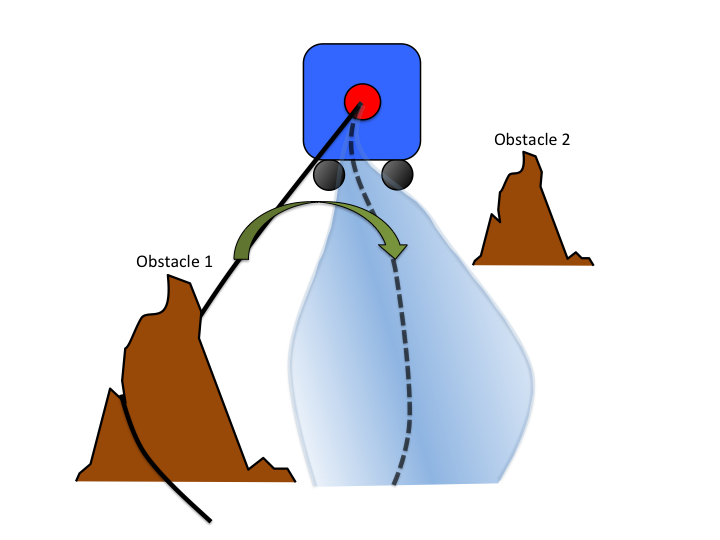
\includegraphics[width=0.48\textwidth, left]{cable_uncertainty}
  \end{center}
  \vspace{-0.5in}
  \label{fig:cable}
  \caption{Employing coordinated control between base and exploratory rovers, we are able to relieve the snagged cable (green arrow) but in doing so are left with uncertainty about where the cable now lies (blue region).}
\end{wrapfigure}
\vspace{-0.15in}

Once the tether has been freed from its constrained state, we find ourselves in a better position to achieve scientific mission objectives but likely also are faced with additional uncertainty as to where the tether (and perhaps the rover itself) is actually currently located \ref{fig:cable}. This uncertainty necessitates planning over a distribution of current and future states (i.e., planning in belief space), and can best be mitigated by searching for and moving toward observations which most reduce the uncertainty in our distribution over the current state of the robot and tether system. In practice this would likely mean moving toward the edges of our believed reachable workspace (in \ref{fig:cable}, to the right of obstacle 2) and using force sensing readings to determine at what point the cable becomes taut against the obstacle. 

By first reducing as much as possible the uncertainty in the current state of the rover and that of the cable, we can then proceed to plan in this optimized belief space in order to achieve mission objectives. This problem can be approached in a number of ways. For simple tasks amenable to a large amount of discretization in both the state and observations, we could formulate this as a partially-observable Markov decision process (POMDP) problem and use an efficient POMDP solver. On the contrary, we could employ efficient sampling-based motion planning methods in conjunction with a particle filter in order to operate directly in continuous space. Depending on the complexity of the systems and terrain involved, planning for such a system in belief space could allow for the possibility to leverage foundational work on robotic motion planning with tether constraints on a planar surface, and bring this work into three-dimensional space by, e.g., casting the problem in 2D and using computational geometry solutions to bias our search for feasible motion plans in 3D. 






% ----------------end of document body---------------------

%---------------- start of references------------------

% \begin{thebibliography}{999}
% \bibitem[Faires \& Burden(1998)]{Faires}{Faires.D.J \& Burden.R. (1998). \textit{Numerical methods: second edition}. USA: Brooks/Cole Publishing Company}
% \bibitem[Griffiths \& Highams(2010)]{Griffiths}{Griffiths.D.F. \& Highams.D.J.(2010). \textit{Numerical methods for Ordinary Differential equations: Initial Value Problems}. London: Springer Undergraduate Mathematics series.}
% % ---Not currently cited but kept in for future referance----\bibitem[Lambert(1973)]{Lambert1973}{Lambert.J.D.(1973). \textit{Computation Methods in Ordinary Differential Equations}, New York: John Wiley \& Sons.}
% \bibitem[Lambert(1991)]{Lambert1991}{Lambert.J.D.(1991). \textit{Numerical Methods for Ordinary Differential Systems: The Initial Value Problem}, West Sussex: John Wiley \& Sons Ltd.}

% \end{thebibliography}

%---------------- end of references------------------


\end{document}